% C-DAWN Stage 1 technical report. Build: tectonic report.tex  (figures: python3 make_figures.py)
\documentclass[10pt,a4paper,twocolumn]{article}

% ---------------------------------------------------------------- page
\usepackage[a4paper,top=21mm,bottom=20mm,left=15.5mm,right=15.5mm,
            columnsep=6mm,headheight=12pt,headsep=4.5mm,footskip=7mm]{geometry}
\usepackage[T1]{fontenc}
\usepackage{amsmath}
\usepackage{newtxtext,newtxmath}
\setsansfont{texgyreheros}[Extension=.otf,UprightFont=*-regular,BoldFont=*-bold,ItalicFont=*-italic,BoldItalicFont=*-bolditalic,Scale=0.9]
\usepackage{microtype}
\usepackage[table]{xcolor}
\usepackage{graphicx,booktabs,tabularx,array,multirow}
\usepackage{tikz}
\usetikzlibrary{arrows.meta,positioning,shapes.geometric,shapes.misc,fit,calc,backgrounds}
\usepackage{fancyhdr,lastpage,eso-pic}
\usepackage{titlesec}
\usepackage[font=footnotesize,labelfont={bf,sf},labelsep=period,justification=justified,singlelinecheck=false,skip=4pt]{caption}
\usepackage{algorithm}
\usepackage[noend]{algpseudocode}
\usepackage[most]{tcolorbox}
\usepackage{enumitem}
\usepackage{stfloats}
\usepackage[hidelinks]{hyperref}

\definecolor{ink}{HTML}{1B1B19}
\definecolor{ink2}{HTML}{55544E}
\definecolor{rule}{HTML}{A9A69C}
\definecolor{faint}{HTML}{F3F1EA}
\definecolor{cblue}{HTML}{2A78D6}
\definecolor{corange}{HTML}{EB6834}
\definecolor{cviolet}{HTML}{4A3AA7}
\definecolor{cred}{HTML}{C0392B}
\definecolor{lblue}{HTML}{E8F0FB}
\definecolor{lorange}{HTML}{FDE7DC}
\definecolor{lviolet}{HTML}{ECEAF7}

\hypersetup{colorlinks=false}
\makeatletter
\renewcommand\normalsize{\@setfontsize\normalsize{9.6}{11.45}%
  \abovedisplayskip 4pt plus 1pt minus 1pt\belowdisplayskip 4pt plus 1pt minus 1pt%
  \abovedisplayshortskip 2pt\belowdisplayshortskip 3pt\let\@listi\@listI}
\makeatother
\normalsize
\setlength{\parskip}{0pt}
\setlength{\parindent}{1.1em}
\setlength{\textfloatsep}{8pt plus 2pt minus 2pt}
\setlength{\floatsep}{7pt plus 2pt minus 2pt}
\setlength{\dbltextfloatsep}{8pt plus 2pt minus 2pt}
\setlength{\abovedisplayskip}{4pt plus 1pt minus 1pt}
\setlength{\belowdisplayskip}{4pt plus 1pt minus 1pt}
\setlength{\abovedisplayshortskip}{2pt}
\setlength{\belowdisplayshortskip}{3pt}
\renewcommand{\topfraction}{0.9}
\renewcommand{\bottomfraction}{0.8}
\renewcommand{\textfraction}{0.08}
\renewcommand{\floatpagefraction}{0.85}
\renewcommand{\dbltopfraction}{0.9}
\renewcommand{\dblfloatpagefraction}{0.85}
\setcounter{topnumber}{3}
\setcounter{dbltopnumber}{2}
\setcounter{totalnumber}{5}
\setlist{nosep,leftmargin=1.3em}

% ---------------------------------------------------------------- border, header, footer
\AddToShipoutPictureBG{%
  \begin{tikzpicture}[remember picture,overlay]
    \draw[line width=0.8pt,color=ink2]
      ([xshift=8.5mm,yshift=-9mm]current page.north west) rectangle
      ([xshift=-8.5mm,yshift=8.5mm]current page.south east);
    \draw[line width=0.3pt,color=rule]
      ([xshift=9.7mm,yshift=-10.2mm]current page.north west) rectangle
      ([xshift=-9.7mm,yshift=9.7mm]current page.south east);
  \end{tikzpicture}}

\pagestyle{fancy}
\fancyhf{}
\fancyhead[L]{\footnotesize\itshape\color{ink2}C-DAWN: a connected, battery-aware UAV swarm for disaster valleys}
\fancyhead[R]{\footnotesize\sffamily\color{ink2}PUSHPAK Grand Challenge 2026 \,|\, UAV-X \,|\, Stage 1}
\fancyfoot[C]{\footnotesize\sffamily\color{ink2}Page \thepage\ of \pageref{LastPage}}
\renewcommand{\headrulewidth}{0.4pt}
\renewcommand{\headrule}{\color{rule}\hrule height\headrulewidth width\headwidth}
\fancypagestyle{first}{\fancyhf{}\renewcommand{\headrulewidth}{0pt}%
  \fancyfoot[C]{\footnotesize\sffamily\color{ink2}Page \thepage\ of \pageref{LastPage}}}

% ---------------------------------------------------------------- headings
\newcommand{\secbox}[1]{\parbox[b]{\linewidth}{\thesection\hspace{0.7em}\MakeUppercase{#1}\\[-1.1ex]{\color{rule}\rule{\linewidth}{0.5pt}}}}
\newcommand{\secboxnn}[1]{\parbox[b]{\linewidth}{\MakeUppercase{#1}\\[-1.1ex]{\color{rule}\rule{\linewidth}{0.5pt}}}}
\titleformat{\section}{\sffamily\bfseries\small\color{ink}}{}{0pt}{\secbox}
\titleformat{name=\section,numberless}{\sffamily\bfseries\small\color{ink}}{}{0pt}{\secboxnn}
\titlespacing*{\section}{0pt}{2.1ex plus .4ex minus .2ex}{0.9ex}
\titleformat{\subsection}{\sffamily\bfseries\footnotesize\color{ink}}{\thesubsection}{0.6em}{}
\titlespacing*{\subsection}{0pt}{1.4ex plus .3ex minus .2ex}{0.5ex}
\titleformat{\paragraph}[runin]{\bfseries}{}{0pt}{}
\titlespacing*{\paragraph}{0pt}{0.5ex}{0.5em}

% ---------------------------------------------------------------- tikz styles
\tikzset{
  >={Stealth[length=1.7mm,width=1.25mm]},
  every picture/.style={line width=0.5pt,draw=ink,font=\sffamily\scriptsize},
  bx/.style={draw=ink,fill=white,rounded corners=1.2pt,align=center,inner sep=2pt},
  bxb/.style={bx,draw=cblue,fill=lblue},
  bxo/.style={bx,draw=corange,fill=lorange},
  bxv/.style={bx,draw=cviolet,fill=lviolet},
  bxg/.style={bx,fill=faint},
  term/.style={bx,fill=faint,rounded corners=2.5mm},
  dec/.style={diamond,draw=ink,fill=white,aspect=2.3,inner sep=0.4pt,align=center},
  arr/.style={->,draw=ink},
  lab/.style={font=\sffamily\tiny,text=ink2},
  yes/.style={font=\sffamily\tiny\bfseries,text=ink},
}

\newcommand{\figrule}{}
\captionsetup[figure]{name=Fig.}

\begin{document}
\thispagestyle{first}

% ================================================================= title block
\twocolumn[{%
\begin{center}
{\sffamily\scriptsize\color{ink2}\MakeUppercase{Technical Report \,\textbar\, Stage 1 \,\textbar\, PUSHPAK Grand Challenge 2026 \,\textbar\, Grand Challenge 1: UAV-X, Resilient BVLOS Swarm}}\\[2.2mm]
{\LARGE\bfseries C-DAWN: Keeping a Battery-Limited UAV Swarm Connected\\[0.8mm] While It Surveys a Himalayan Disaster Valley}\\[2.6mm]
{\normalsize Team C-DAWN \quad\textbar\quad [Member names] \quad\textbar\quad [Institution, City]}\\[0.8mm]
{\footnotesize\itshape\color{ink2}Source code: github.com/paramvansh01/drone\_swarm \quad\textbar\quad Simulation track \quad\textbar\quad 26 September 2026}
\end{center}
\vspace{-1mm}
\begin{tcolorbox}[enhanced,colback=faint,colframe=ink,boxrule=0pt,leftrule=2.2pt,arc=0pt,
  left=3mm,right=3mm,top=1.6mm,bottom=1.6mm,fontupper=\small]
{\sffamily\bfseries\footnotesize ABSTRACT.}\;
When an earthquake or a landslide cuts the road and the towers in a Himalayan valley, the first hours depend on two things: getting eyes on the damaged sites, and getting what those eyes see back to the people running the response. We built C-DAWN, a simulation-first autonomy stack for a fleet of battery-limited quadrotors that fly from a ground control station (GCS) outside the affected area. The swarm works out from the terrain how many relays it needs, uses an E(3)-equivariant graph network and a differentiable radio model to decide where they hover, hands a relay station to a fresh aircraft \emph{before} the tired one leaves to swap its battery, and drops lower-priority work when a new emergency is reported. It is never told about a failure. It notices one from heartbeats, acknowledgements, noise readings and battery current, the same evidence a fielded swarm would have, and a causal model with small altitude experiments tells terrain shadow apart from interference. Across four scenarios, two of them on real terrain at Kedarnath and Uttarkashi, with 4 to 11 hidden disturbances each, C-DAWN delivered 97.3\% of survey tasks, 96.7\% of packets and 95.3\% connectivity, against 87.8\%, 91.6\% and 88.6\% for a fixed-role baseline. Neither had a collision, a geofence violation or a flat battery.

\vspace{1mm}
{\footnotesize\color{ink2}\textbf{Keywords:} UAV swarm, BVLOS, multi-hop relay, equivariant graph neural network, differentiable RF, structural causal model, energy-aware planning, delay-tolerant networking}
\end{tcolorbox}
\vspace{1.5mm}
\begin{center}
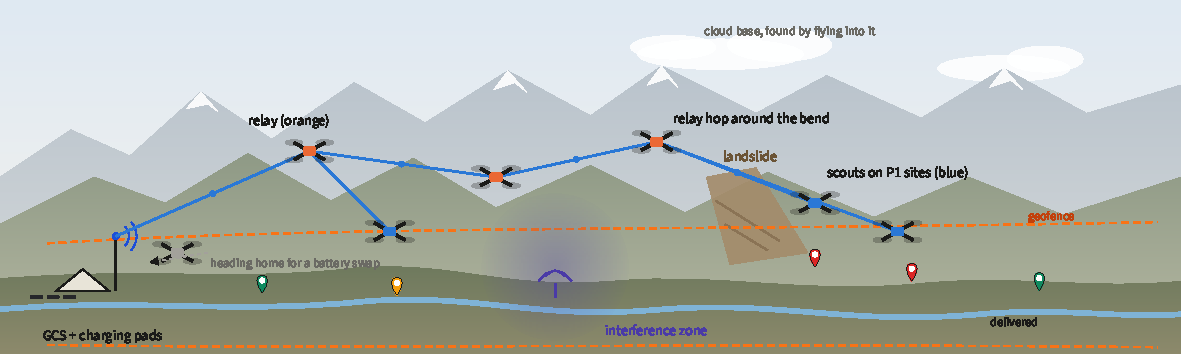
\includegraphics[width=\textwidth]{figs/fig_teaser.pdf}
\end{center}
\vspace{-2mm}
{\footnotesize\textsf{\textbf{Fig. 1.}} What C-DAWN is doing. The GCS sits at the valley mouth with its charging pads. Relays (orange) hold a chain that follows the valley round its bend; scouts (blue) survey the reported sites, coloured by priority, which turn green once their data has reached the GCS. One aircraft is heading back for a battery swap while its station stays covered. The interference zone, the cloud base and the geofence are all things the swarm has to find out about or respect on its own.}
\vspace{3mm}
}]
\setcounter{figure}{1}

% ================================================================= 1
\section{Introduction}
Mountain valleys are hard places to keep a radio link alive. A 900\,MHz link at half a watt reaches tens of kilometres in open air, but in the Mandakini or Bhagirathi valleys one spur of rock can take 40\,dB out of it. Add a battery that lasts a quarter of an hour, a valley wind that makes the trip home twice as slow as the trip out, and the ordinary ways a deployment goes wrong (an aircraft goes down, a radio dies, somebody's generator sprays noise across the band), and the UAV-X problem comes into focus. The fleet has to survey every reported site and keep talking to the GCS the whole time, without anyone telling it what has just broken.

Most multi-UAV search systems [11] plan the survey first and check the radio afterwards. We treat communication as part of the mission instead. A site only counts as done when its imagery has reached the GCS, so the swarm is scored on exactly what responders need. Our contributions are:
\begin{enumerate}
  \item A \textbf{terrain-aware relay requirement}: a chain walk over the elevation map decides how many relays the valley needs, instead of a constant.
  \item \textbf{Learned relay placement}: an E(3)-equivariant graph network trained without labels through a differentiable terrain and link model, then polished by gradient steps at run time.
  \item \textbf{Dynamic roles} with 200 to 300\,ms failover and a \textbf{make-before-break handover}, so a relay leaving to recharge never opens a gap.
  \item \textbf{Energy- and wind-aware planning} driven by each aircraft's own measured current draw.
  \item A \textbf{perception-only awareness layer} with causal link diagnosis. The autonomy never reads simulator truth, and a test audits the source to keep it that way.
  \item A reproducible evaluation: JSON scenarios, hidden disturbances, standard logs and a fixed-role baseline.
\end{enumerate}

% ================================================================= 2
\section{Problem and System Model}
\paragraph{Area and GCS.} The affected area is a valley corridor about 4.2\,km long inside a 5.1\,$\times$\,5.1\,km terrain tile. The GCS is a fixed node at the valley mouth with its antenna on a 10\,m mast and a row of charging pads. It cannot fail, every packet is going there, and every sortie starts and ends on one of its pads.

\paragraph{Fleet.} Five or six identical 1.9\,kg quadrotors with a 900\,MHz mesh radio (27\,dBm, 3\,dBi). Hover endurance is about 18 minutes and cruise about 15; a battery swap takes up to two minutes. Roles are not fixed: an aircraft can be a scout, a relay, or on standby.

\paragraph{Tasks.} A survey task $p$ has a position, a priority $\pi_p\in\{1,2,3\}$ with weight $w_p=3,2,1$, and a release time. Tasks released after launch are the newly emerging ones, invisible to the swarm until reported. A task is surveyed after a 2\,s dwell within 30\,m and \emph{delivered} when all 12 chunks of its data are at the GCS.

\paragraph{Constraints.} A mission clock of 12 or 15 minutes, a polygon geofence with an AGL ceiling, at least 3\,m between aircraft, and a battery that never runs out in the air. We read ``finish safely within the allotted time'' strictly: every aircraft is back on a pad by the deadline.

\begin{table*}[t]
\centering
\caption{How each UAV-X requirement is met and how we measure it.}
\label{tab:trace}
\footnotesize
\renewcommand{\arraystretch}{1.12}
\begin{tabularx}{\textwidth}{@{}>{\raggedright\arraybackslash}p{30mm}>{\raggedright\arraybackslash}X>{\raggedright\arraybackslash\ttfamily\scriptsize}p{31mm}>{\raggedright\arraybackslash}p{37mm}@{}}
\toprule
\textsf{\textbf{The swarm must}} & \textsf{\textbf{What C-DAWN does}} & \normalfont\textsf{\textbf{Where}} & \textsf{\textbf{Measured as}}\\
\midrule
Survey all assigned locations & Assign a task only if the aircraft can reach it, survey it and get home inside its battery and the clock; greedy on priority weight per second of travel (Sec.~\ref{sec:alloc}). & sim/guidance.py sim/energy.py & completion rate and time, priority-weighted score\\
Keep end-to-end comms with the GCS & GCS as a fixed graph node; chain sized from terrain; GNN placement; causal-aware routing; store-and-forward traffic. & mesh/roles.py gnn/ mesh/traffic.py & PDR, latency, availability, downtime\\
Assign relays dynamically & Relay count re-planned every second; launch from pads first, else promote the scout doing the least valuable work. & mesh/roles.py & relay reallocations, reconfiguration efficiency\\
Reconfigure on degradation, failure or recharge & Heartbeat failover; interference localised and routed round; make-before-break handover; lost-link failsafe. & mesh/election.py mesh/interference.py & recovery time, performance after faults\\
Prioritise new high-priority regions & A new P1 task pre-empts the best-placed scout on lower-priority work; standby scouts; discretionary returns turned round. & sim/guidance.py & emergency response time, weighted score\\
Finish safely, on time & Energy-aware return; home before the deadline; geofence projection on every setpoint; predictive separation; spaced take-offs. & sim/deconfliction.py sim/world.py & collisions, minimum separation, flat batteries, geofence breaches\\
\bottomrule
\end{tabularx}
\end{table*}

% ================================================================= 3
\section{Architecture}
Everything runs in one Python process on one simulated clock. The live console, a three-laptop demonstration and the headless benchmark all call the same \texttt{step()}, so the numbers in Section~\ref{sec:eval} come from the code that is shown live. Fig.~\ref{fig:arch} shows the layers. The line we care most about is the dashed one. Below it is the simulator, which knows everything. Above it is the autonomy, which only knows what its sensors and its radio tell it. Measurements are the only thing that crosses upward, and setpoints are the only thing that crosses back down.

\begin{figure*}[t]
\centering
\resizebox{\textwidth}{!}{%
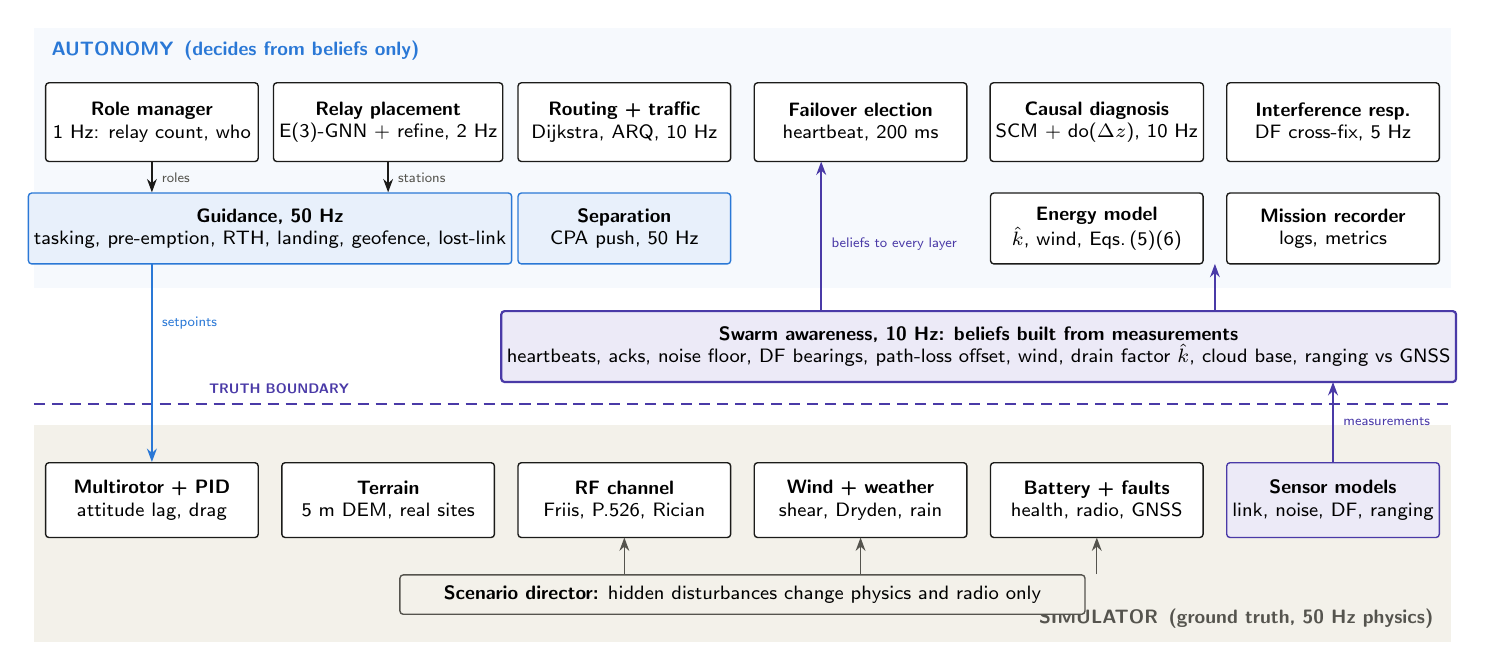
\begin{tikzpicture}[x=1mm,y=1mm]
  % bands
  \fill[lblue!40] (0,18) rectangle (180,51);
  \fill[faint] (0,-27) rectangle (180,0.5);
  \node[anchor=north west,font=\sffamily\scriptsize\bfseries,text=cblue] at (1,50.6) {AUTONOMY \,(decides from beliefs only)};
  \node[anchor=south east,font=\sffamily\scriptsize\bfseries,text=ink2] at (179,-26.6) {SIMULATOR \,(ground truth, 50 Hz physics)};
  % row 1
  \node[bx,minimum width=27mm,minimum height=10mm] (rm)  at (15,39)  {\textbf{Role manager}\\1 Hz: relay count, who};
  \node[bx,minimum width=27mm,minimum height=10mm] (gnn) at (45,39)  {\textbf{Relay placement}\\E(3)-GNN + refine, 2 Hz};
  \node[bx,minimum width=27mm,minimum height=10mm] (rt)  at (75,39)  {\textbf{Routing + traffic}\\Dijkstra, ARQ, 10 Hz};
  \node[bx,minimum width=27mm,minimum height=10mm] (el)  at (105,39) {\textbf{Failover election}\\heartbeat, 200 ms};
  \node[bx,minimum width=27mm,minimum height=10mm] (scm) at (135,39) {\textbf{Causal diagnosis}\\SCM + do($\Delta z$), 10 Hz};
  \node[bx,minimum width=27mm,minimum height=10mm] (ir)  at (165,39) {\textbf{Interference resp.}\\DF cross-fix, 5 Hz};
  % row 2
  \node[bxb,minimum width=57mm,minimum height=9mm] (gd) at (30,25.5) {\textbf{Guidance, 50 Hz}\\tasking, pre-emption, RTH, landing, geofence, lost-link};
  \node[bxb,minimum width=27mm,minimum height=9mm] (sep) at (75,25.5) {\textbf{Separation}\\CPA push, 50 Hz};
  \node[bx,minimum width=27mm,minimum height=9mm] (en) at (135,25.5) {\textbf{Energy model}\\$\hat k$, wind, Eqs.\,(5)(6)};
  \node[bx,minimum width=27mm,minimum height=9mm] (rec) at (165,25.5) {\textbf{Mission recorder}\\logs, metrics};
  % awareness
  \node[bxv,minimum width=117mm,minimum height=9mm,line width=0.8pt] (aw) at (120,10.5) {\textbf{Swarm awareness, 10 Hz: beliefs built from measurements}\\heartbeats, acks, noise floor, DF bearings, path-loss offset, wind, drain factor $\hat k$, cloud base, ranging vs GNSS};
  % boundary
  \draw[cviolet,line width=1pt,dash pattern=on 4pt off 2.5pt] (0,3.2) -- (180,3.2);
  \node[anchor=south west,font=\sffamily\tiny\bfseries,text=cviolet] at (21,3.3) {TRUTH BOUNDARY};
  % simulator row
  \node[bx,minimum width=27mm,minimum height=9.5mm] (fc) at (15,-9)  {\textbf{Multirotor + PID}\\attitude lag, drag};
  \node[bx,minimum width=27mm,minimum height=9.5mm] (tr) at (45,-9)  {\textbf{Terrain}\\5 m DEM, real sites};
  \node[bx,minimum width=27mm,minimum height=9.5mm] (rf) at (75,-9)  {\textbf{RF channel}\\Friis, P.526, Rician};
  \node[bx,minimum width=27mm,minimum height=9.5mm] (wd) at (105,-9) {\textbf{Wind + weather}\\shear, Dryden, rain};
  \node[bx,minimum width=27mm,minimum height=9.5mm] (bt) at (135,-9) {\textbf{Battery + faults}\\health, radio, GNSS};
  \node[bxv,minimum width=27mm,minimum height=9.5mm] (sm) at (165,-9) {\textbf{Sensor models}\\link, noise, DF, ranging};
  \node[bxg,minimum width=87mm,minimum height=5mm,draw=ink2] (sd) at (90,-21) {\textbf{Scenario director:} hidden disturbances change physics and radio only};
  % arrows
  \draw[arr] (rm.south) -- node[right,lab]{roles} (rm.south |- gd.north);
  \draw[arr] (gnn.south) -- node[right,lab]{stations} (gnn.south |- gd.north);
  \draw[arr,cblue,line width=0.8pt] (15,21) -- node[right,lab,text=cblue,pos=0.3]{setpoints} (fc.north);
  \draw[arr,cviolet,line width=0.8pt] (sm.north) -- node[right,lab,text=cviolet]{measurements} (165,6);
  \draw[arr,cviolet,line width=0.8pt] (100,15) -- node[right,lab,text=cviolet,pos=0.45]{beliefs to every layer} (100,34);
  \draw[arr,cviolet] (aw.north -| 150,0) ++(0,0) -- (150,15) -- (150,21);
  \foreach \x in {75,105,135} \draw[arr,ink2] (sd.north -| \x,0) -- (\x,-13.75);
\end{tikzpicture}}
\caption{Layers, rates and the truth boundary. The simulator owns terrain, flight physics, the radio channel, faults and the scenario's hidden disturbances. Only sensor readings cross the purple line. The awareness layer turns them into beliefs and every autonomy layer decides from those. Setpoints are the only thing that goes back down. Rates are per simulated second.}
\label{fig:arch}
\end{figure*}

% ================================================================= 4
\section{Simulation Environment}
\paragraph{Terrain.} Each site is a 5.1\,km terrain pack with a 5\,m elevation grid built from AWS Open Data terrain tiles (SRTM and Copernicus derived) and Sentinel-2 cloudless imagery [9,\,10]. We ship four real disaster sites (Kedarnath, Uttarkashi, Joshimath and Chungthang) and a procedural valley for repeatable tests. The mission corridor is found by dynamic programming along the valley floor.

\paragraph{Flight.} An underactuated multirotor with attitude lag, slew limits and airspeed drag, flown by a cascaded PID. Wind follows a power-law shear, $w(z)=w_{\mathrm{ref}}(z/z_{\mathrm{ref}})^{0.16}$, with Dryden turbulence and gusts [8].

\paragraph{Radio.} Every tick, every pair of aircraft and every aircraft-to-GCS link gets a link budget
\begin{equation}
P_r = P_t + G_t + G_r - L_{\mathrm{fs}}(d) - J(v) - L_x,\qquad \mathrm{SNR}=P_r-N,
\label{eq:budget}
\end{equation}
where $L_{\mathrm{fs}}$ is Friis free-space loss [2], $L_x$ extra loss (wet antennas in rain) and $J(v)$ the ITU-R P.526 knife-edge loss over the worst ridge on the path [1]. With $h$ the height of the ridge above the ray and $d_1,d_2$ its distances to the two ends,
\begin{equation}
\begin{gathered}
J(v)=6.9+20\log_{10}\!\Big(\sqrt{(v-0.1)^2+1}+v-0.1\Big),\\
v=h\,\sqrt{2(d_1+d_2)/(\lambda\, d_1 d_2)}.
\end{gathered}
\label{eq:knife}
\end{equation}
The noise floor $N$ is thermal plus any interference received from active sources. Packet delivery is averaged over a burst of 24 packets, each with its own Rician fade ($K=6$\,dB). We learnt early that one fading draw per tick makes a steady link look like it is flapping, which confused both routing and the causal engine.

% ================================================================= 5
\section{Mission Autonomy}
Before the individual pieces, it helps to see one aircraft's life (Fig.~\ref{fig:life}). It starts charged on a pad, launches as a scout or a relay, may swap roles in the air, and eventually comes home for one of five reasons. It lands, has its battery swapped and waits until the role manager needs it again. Everything in this section decides when one of these arrows is taken.

\begin{figure}[t]
\centering
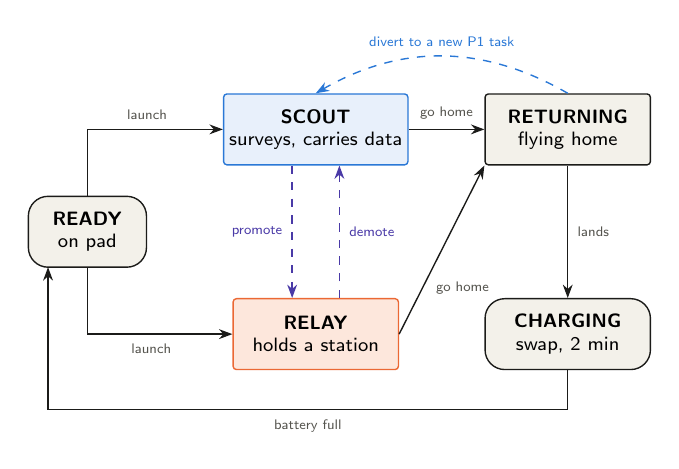
\begin{tikzpicture}[x=1mm,y=1mm]
  \node[term,minimum width=15mm,minimum height=9mm] (rd) at (0,0) {\textbf{READY}\\on pad};
  \node[bxb,minimum width=21mm,minimum height=9mm] (sc) at (29,13) {\textbf{SCOUT}\\surveys, carries data};
  \node[bxo,minimum width=21mm,minimum height=9mm] (rl) at (29,-13) {\textbf{RELAY}\\holds a station};
  \node[bxg,minimum width=21mm,minimum height=9mm] (rt) at (61,13) {\textbf{RETURNING}\\flying home};
  \node[term,minimum width=21mm,minimum height=9mm] (ch) at (61,-13) {\textbf{CHARGING}\\swap, 2 min};
  \draw[arr] (rd.north) |- node[pos=0.72,above,lab]{launch} (sc.west);
  \draw[arr] (rd.south) |- node[pos=0.72,below,lab]{launch} (rl.west);
  \draw[arr,cviolet,dashed] ([xshift=-3mm]sc.south) -- node[left,lab,text=cviolet]{promote} ([xshift=-3mm]rl.north);
  \draw[arr,cviolet,dashed] ([xshift=3mm]rl.north) -- node[right,lab,text=cviolet]{demote} ([xshift=3mm]sc.south);
  \draw[arr] (sc.east) -- node[above,lab]{go home} (rt.west);
  \draw[arr] (rl.east) -- node[pos=0.35,below right=-0.5mm,lab]{go home} (rt.south west);
  \draw[arr] (rt.south) -- node[right,lab]{lands} (ch.north);
  \draw[arr] (ch.south) -- ++(0,-5) -| node[pos=0.25,below,lab]{battery full} (-5,-4.5);
  \draw[arr,cblue,dashed] (rt.north) to[out=150,in=30] node[above,lab,text=cblue]{divert to a new P1 task} (sc.north);
\end{tikzpicture}
\caption{The life of one aircraft. Dashed purple arrows are role changes in flight, each logged as a reallocation. An aircraft goes home for its energy threshold, the mission clock, a lost link, lack of work, or a completed handover. Failure is not a state anyone announces: an aircraft nobody has heard for 200\,ms is treated as gone.}
\label{fig:life}
\end{figure}

\subsection{Energy and time, before anything else}
Every decision that sends an aircraft away from the GCS has to be affordable. Drain follows the airframe's power law, scaled by a factor $\hat k$ that each aircraft \emph{measures} as the ratio of its battery current to what its thrust should need, over a 15\,s window:
\begin{gather}
\dot b=\hat k\,[\,b_0+(b_1-b_0)f_T\,],\quad v_g=\mathrm{clip}(v_a+\hat{\mathbf w}\!\cdot\!\hat{\mathbf u},5,19),\label{eq:drain}\\
\hat k \leftarrow \hat k + \tfrac{\Delta t}{15}\big(I_{\mathrm{meas}}/I_{\mathrm{nom}}-\hat k\big),\label{eq:khat}
\end{gather}
with $f_T$ the thrust fraction, $\hat{\mathbf w}$ the swarm's wind estimate at cruise height and $\hat{\mathbf u}$ the direction of travel. A damaged motor raises $I_{\mathrm{meas}}$, so $\hat k$ rises and the aircraft plans more conservatively without being told anything. Leg time is $T(a,b)=1.15\,|ab|/v_g+25$\,s. With safety factor $s=1.2$ and an 8\% landing reserve, the return and handover thresholds are
\begin{gather}
B_{\mathrm{rth}}=\max\!\big(12,\ s\,\dot b\,T(\mathbf p,\mathbf h)+8\big),\label{eq:rth}\\
B_{\mathrm{ho}}=B_{\mathrm{rth}}+s\,\dot b_{\mathrm{hov}}\big(T(\mathbf g,\mathbf q)+25\,\mathrm{s}\big),\label{eq:ho}
\end{gather}
where $\mathbf p$ is the aircraft, $\mathbf h$ its pad, $\mathbf g$ the GCS and $\mathbf q$ a relay's station. There is no fixed ``come home at 22\%'' rule. A relay four kilometres up the valley with the wind in its face turns for home at about 62\%, one next to the GCS at 12\% (Fig.~\ref{fig:energy}).

\begin{figure}[t]
\centering
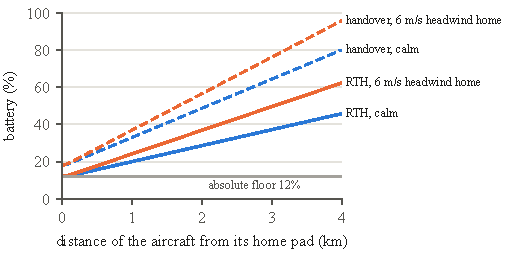
\includegraphics[width=\columnwidth]{figs/fig_energy.pdf}
\caption{Thresholds from Eqs.~(\ref{eq:rth}) and (\ref{eq:ho}) for a cruising aircraft. A headwind on the way home adds 16 points at 4\,km. Dashed lines are handover thresholds, which leave time for a replacement to fly out.}
\label{fig:energy}
\end{figure}

\subsection{Who surveys what, and when to change our mind}\label{sec:alloc}
Allocation is greedy on value rate. At each step we take the (scout, task) pair with the largest value rate
\begin{equation}
V_{s,p}=\frac{w_p}{\mathrm{ETA}_{s,p}+60\,\mathrm{s}},
\label{eq:value}
\end{equation}
considered only if the task is affordable and the round trip fits in the time left. The 60\,s term stops a very close P3 task from always beating a P1 task a little further away. When a P1 task arrives and no idle scout can take it, the best-placed scout on lower-priority work is pre-empted, unless it is already hovering over its target. Idle scouts with a healthy battery loiter at a standby point mid-valley, inside relay cover, so the next emergency is minutes closer. A scout flying home only because it had nothing to do can be turned round. Fig.~\ref{fig:alloc} is the whole loop.

\begin{figure}[t]
\centering
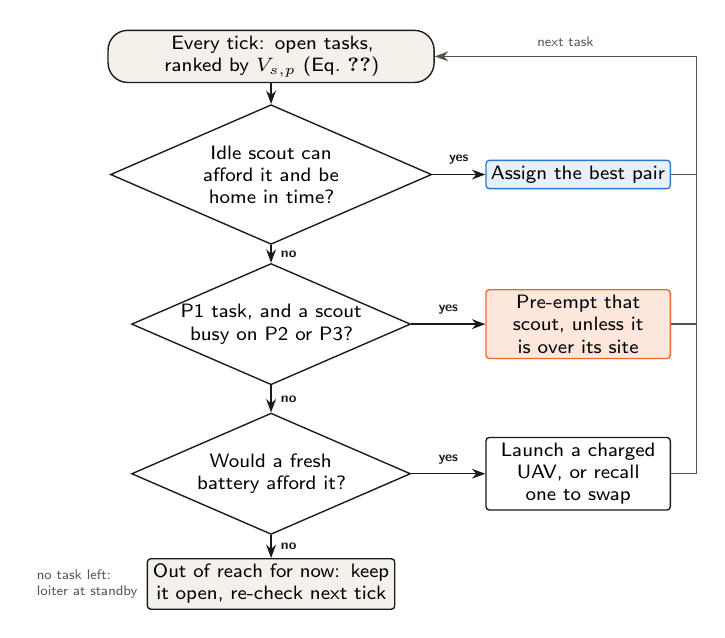
\begin{tikzpicture}[x=1mm,y=1mm,node distance=4mm]
  \node[term,text width=40mm] (st) at (0,0) {Every tick: open tasks, ranked by $V_{s,p}$ (Eq.~\ref{eq:value})};
  \node[dec,text width=23mm] (d1) at (0,-15) {Idle scout can afford it and be home in time?};
  \node[dec,text width=23mm] (d2) at (0,-34) {P1 task, and a scout busy on P2 or P3?};
  \node[dec,text width=23mm] (d3) at (0,-53) {Would a fresh battery afford it?};
  \node[bxg,text width=30mm] (en) at (0,-67) {Out of reach for now: keep it open, re-check next tick};
  \node[bxb,text width=22mm] (r1) at (39,-15) {Assign the best pair};
  \node[bxo,text width=22mm] (r2) at (39,-34) {Pre-empt that scout, unless it is over its site};
  \node[bx,text width=22mm] (r3) at (39,-53) {Launch a charged UAV, or recall one to swap};
  \draw[arr] (st) -- (d1);
  \draw[arr] (d1) -- node[right,yes]{no} (d2);
  \draw[arr] (d2) -- node[right,yes]{no} (d3);
  \draw[arr] (d3) -- node[right,yes]{no} (en);
  \draw[arr] (d1) -- node[above,yes]{yes} (r1);
  \draw[arr] (d2) -- node[above,yes]{yes} (r2);
  \draw[arr] (d3) -- node[above,yes]{yes} (r3);
  \draw[ink2] (r1.east) -- (54,-15);
  \draw[ink2] (r2.east) -- (54,-34);
  \draw[ink2] (r3.east) -- (54,-53);
  \draw[arr,ink2] (54,-53) -- (54,0) -- node[above,lab]{next task} (st.east);
  \node[lab,align=left,anchor=west] at (-31,-67) {no task left:\\loiter at standby};
\end{tikzpicture}
\caption{Task allocation, run every tick. ``Afford'' means battery for the task, the trip home and the landing reserve; ``in time'' means the round trip fits before the deadline.}
\label{fig:alloc}
\end{figure}

\subsection{How many relays the terrain asks for}
This replaces a guess with a measurement of the mountain. Once a second the role manager collects the points where work is happening: scouts on task, open reachable tasks, aircraft carrying undelivered data and aircraft still flying home. For the farthest of them it walks the chain in Algorithm~\ref{alg:chain}.

\begin{algorithm}[t]
\caption{Terrain-aware relay chain}\label{alg:chain}
\footnotesize
\begin{algorithmic}[1]
\Require GCS antenna $\mathbf g$, farthest work point $\mathbf t$, elevation map, noise estimate $\hat N$, localised sources $\hat{\mathcal S}$
\State sample the valley centreline every 60\,m from $\mathbf g$ to $\mathbf t$ at 160\,m AGL
\State $\mathbf c\gets\mathbf g$;\ hops $\gets[\,]$
\While{$\mathrm{SNR}(\mathbf c,\mathbf t)<15$\,dB}\Comment{Eq.~(\ref{eq:budget}) over the map}
  \State $\mathbf s\gets$ farthest sample with $\mathrm{SNR}(\mathbf c,\mathbf s)\ge15$\,dB given $\hat N,\hat{\mathcal S}$
  \If{no such $\mathbf s$} \textbf{break} \EndIf
  \State append $\mathbf s$ to hops;\ $\mathbf c\gets\mathbf s$
\EndWhile
\State \Return $|$hops$|$ (relay requirement) and hops (GNN anchors)
\end{algorithmic}
\end{algorithm}

The 15\,dB target is roughly the 9\,dB a 256-byte frame needs for 95\% delivery, plus fading margin. On Kedarnath the walk gives exactly one relay (Fig.~\ref{fig:chain}): the valley turns south past the 2\,km mark and a spur blocks the straight line from the GCS to the far sites.

The requirement then drives assignment. When there are fewer relays than needed, a charged aircraft on a pad launches first, because it arrives with a full battery. Failing that, the scout doing the least valuable work closest to the missing hop is promoted, and at least one scout always keeps surveying. When there are more relays than needed for 25\,s, the spare goes back to surveying, or home. Every change is logged with its reason; one undone within 30\,s counts as a flap against reconfiguration efficiency.

\begin{figure}[t]
\centering
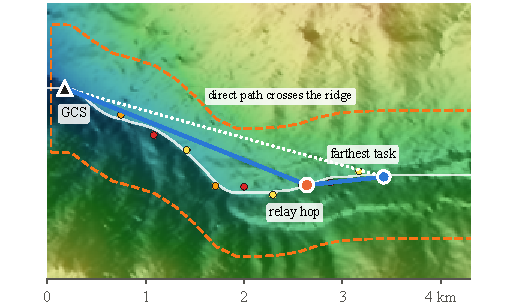
\includegraphics[width=\columnwidth]{figs/fig_chain.pdf}
\caption{Algorithm~\ref{alg:chain} on the real Kedarnath terrain. Blue lines are the planned links; the white dotted line is the direct path, which clips the spur. Dots are survey tasks by priority (red P1, amber P2, yellow P3); the orange dashed line is the geofence.}
\label{fig:chain}
\end{figure}

\subsection{Where the relays hover: an equivariant GNN}\label{sec:gnn}
The role manager decides how many relays and who flies them. Where they hover is decided by a graph network followed by a short gradient polish (Fig.~\ref{fig:gnn}). We picked a learned model for one reason: the placement has to be recomputed twice a second as scouts move, and one forward pass costs only 1.4\,ms.

\paragraph{Graph and features.} Every aircraft that somebody can hear, plus the GCS, is a node; with fewer than ten nodes we use a fully connected graph. Positions $\mathbf x_i\in\mathbb R^3$ are centred on the swarm centroid and divided by $L=250$\,m, because raw coordinates in kilometres saturate an MLP. Each node carries nine invariant features $\mathbf h^0_i$: battery, a one-hot role (scout, relay, GCS), mean and minimum measured link quality, degree, AGL and an interference flag.

\paragraph{Message passing.} After a two-layer SiLU embedding to 64 channels, four E(n)-equivariant layers [3] update features and coordinates together:
\begin{gather}
m_{ij}=\phi_m\big(\mathbf h_i,\mathbf h_j,\|\mathbf x_j-\mathbf x_i\|\big),\label{eq:msg}\\
\mathbf x_i\leftarrow\mathbf x_i+\frac{1}{|\mathcal N_i|}\sum_{j\in\mathcal N_i}(\mathbf x_j-\mathbf x_i)\,\phi_x(m_{ij}),\label{eq:coord}\\
\mathbf h_i\leftarrow\mathbf h_i+\phi_h\Big(\mathbf h_i,\sum_{j}m_{ij}\Big).\label{eq:feat}
\end{gather}
$\phi_m$ and $\phi_h$ are two-layer MLPs and $\phi_x$ ends in a $\tanh$, so each layer's step is bounded. Since the only geometric input to $\phi_m$ is a distance and the coordinate update is a weighted sum of relative vectors, the network satisfies $f(Q\mathbf x+\mathbf t)=Qf(\mathbf x)+\mathbf t$ for any rotation or reflection $Q$ and shift $\mathbf t$. A model trained on one valley therefore works on a valley running in any direction; unit tests check this numerically, to 1\,cm for the full network. We used mean rather than sum aggregation in (\ref{eq:coord}) so the step size does not grow with the number of neighbours.

\paragraph{Output.} A per-node gate $g_i=\sigma(\mathrm{MLP}(\mathbf h_i))$ scales the proposed move, $\Delta_i=g_i L(\tilde{\mathbf x}^{(4)}_i-\tilde{\mathbf x}^{(0)}_i)$, which is clipped to 220\,m and applied to relays only. Scouts, the GCS and a relay that is being relieved stay fixed. The network has 123{,}397 parameters.

\begin{figure*}[t]
\centering
\resizebox{\textwidth}{!}{%
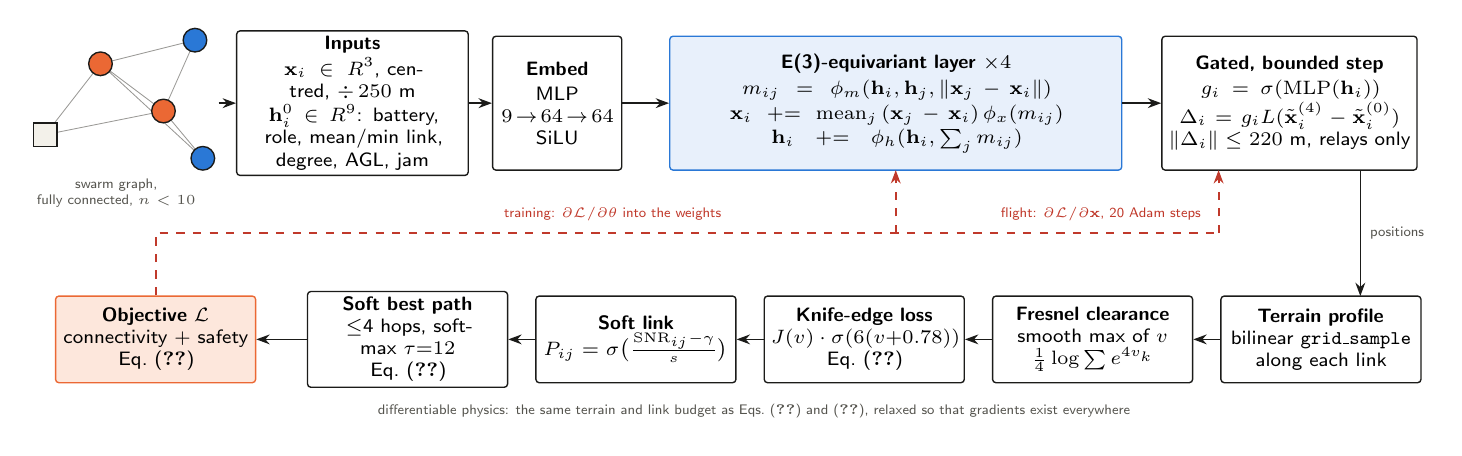
\begin{tikzpicture}[x=1mm,y=1mm]
  % graph sketch
  \draw[ink2!60,line width=0.3pt] (3,36)--(10,45)--(18,39)--(22,48) (18,39)--(23,33) (3,36)--(18,39) (10,45)--(22,48) (10,45)--(23,33);
  \filldraw[fill=faint,draw=ink] (1.5,34.5) rectangle (4.5,37.5);
  \foreach \p in {(10,45),(18,39)} \filldraw[fill=corange,draw=ink] \p circle (1.5);
  \foreach \p in {(22,48),(23,33)} \filldraw[fill=cblue,draw=ink] \p circle (1.5);
  \node[lab,align=center] at (12,28.6) {swarm graph,\\fully connected, $n<10$};
  % top row
  \node[bx,minimum height=17mm,text width=28mm] (in) at (42,40) {\textbf{Inputs}\\[0.4mm]$\mathbf x_i\in\mathbb R^3$, centred, $\div\,250$ m\\[0.3mm]$\mathbf h^0_i\in\mathbb R^9$: battery, role, mean/min link, degree, AGL, jam};
  \node[bx,minimum height=17mm,text width=15mm] (em) at (68,40) {\textbf{Embed}\\[0.4mm]MLP\\$9\!\to\!64\!\to\!64$\\SiLU};
  \node[bxb,minimum height=17mm,text width=56mm] (eg) at (111,40) {\textbf{E(3)-equivariant layer} $\times 4$\\[0.6mm]
      $m_{ij}=\phi_m(\mathbf h_i,\mathbf h_j,\|\mathbf x_j-\mathbf x_i\|)$\\[0.3mm]
      $\mathbf x_i \mathrel{+}= \mathrm{mean}_j\,(\mathbf x_j-\mathbf x_i)\,\phi_x(m_{ij})$\\[0.3mm]
      $\mathbf h_i \mathrel{+}= \phi_h(\mathbf h_i,\textstyle\sum_j m_{ij})$};
  \node[bx,minimum height=17mm,text width=31mm] (gt) at (161,40) {\textbf{Gated, bounded step}\\[0.4mm]$g_i=\sigma(\mathrm{MLP}(\mathbf h_i))$\\$\Delta_i=g_i L(\tilde{\mathbf x}^{(4)}_i-\tilde{\mathbf x}^{(0)}_i)$\\$\|\Delta_i\|\le 220$ m, relays only};
  \draw[arr] (in) -- (em); \draw[arr] (em) -- (eg); \draw[arr] (eg) -- (gt);
  \draw[arr] (25,40) -- (in.west);
  % bottom row (right to left)
  \node[bx,minimum height=11mm,text width=24mm] (b1) at (165,10) {\textbf{Terrain profile}\\bilinear \texttt{grid\_sample}\\along each link};
  \node[bx,minimum height=11mm,text width=24mm] (b2) at (136,10) {\textbf{Fresnel clearance}\\smooth max of $v$\\$\tfrac14\log\sum e^{4v_k}$};
  \node[bx,minimum height=11mm,text width=24mm] (b3) at (107,10) {\textbf{Knife-edge loss}\\$J(v)\cdot\sigma(6(v{+}0.78))$\\Eq.~(\ref{eq:knife})};
  \node[bx,minimum height=11mm,text width=24mm] (b4) at (78,10) {\textbf{Soft link}\\$P_{ij}=\sigma\big(\tfrac{\mathrm{SNR}_{ij}-\gamma}{s}\big)$};
  \node[bx,minimum height=11mm,text width=24mm] (b5) at (49,10) {\textbf{Soft best path}\\$\le$4 hops, softmax $\tau{=}12$\\Eq.~(\ref{eq:path})};
  \node[bxo,minimum height=11mm,text width=24mm] (b6) at (17,10) {\textbf{Objective} $\mathcal L$\\connectivity + safety\\Eq.~(\ref{eq:obj})};
  \draw[arr] (b1) -- (b2); \draw[arr] (b2) -- (b3); \draw[arr] (b3) -- (b4); \draw[arr] (b4) -- (b5); \draw[arr] (b5) -- (b6);
  \draw[arr] (170,31.5) -- node[right,lab]{positions} (170,15.5);
  % gradients
  \draw[cred,dashed,line width=0.7pt] (b6.north) -- (17,23.5) -- (152,23.5);
  \draw[->,cred,dashed,line width=0.7pt] (111,23.5) -- (111,31.5);
  \draw[->,cred,dashed,line width=0.7pt] (152,23.5) -- (152,31.5);
  \node[lab,text=cred,anchor=south west,align=left] at (60,23.8) {training: $\partial\mathcal L/\partial\theta$ into the weights};
  \node[lab,text=cred,anchor=south east,align=right] at (151,23.8) {flight: $\partial\mathcal L/\partial\mathbf x$, 20 Adam steps};
  \node[lab,anchor=north] at (93,3) {differentiable physics: the same terrain and link budget as Eqs.~(\ref{eq:budget}) and (\ref{eq:knife}), relaxed so that gradients exist everywhere};
\end{tikzpicture}}
\caption{Relay placement. Top: the forward pass, from swarm graph to a bounded move for each relay. Bottom: the differentiable link model that scores a layout. Red: gradients. During training they update the network weights; in flight the same gradients move the relay positions for 20 Adam steps (about 21\,ms). No labelled data is used anywhere.}
\label{fig:gnn}
\end{figure*}

\paragraph{A differentiable radio.} To score a layout without labels we rebuilt Eqs.~(\ref{eq:budget}) and (\ref{eq:knife}) in PyTorch so that every step has a gradient. Terrain along each link is read with bilinear \texttt{grid\_sample}. The worst ridge is a hard max, which would send gradient to one sample only, so we use a log-sum-exp smooth max. ITU-R P.526 is only defined for $v>-0.78$, and a hard cutoff would put a kink exactly where relays spend their time (at the edge of Fresnel clearance), so it is gated by a sigmoid. Link delivery becomes $P_{ij}=\sigma((\mathrm{SNR}_{ij}-\gamma)/s)$ with $s=3$\,dB in flight. End-to-end reliability to scout $k$ is a soft Bellman recursion over at most four hops:
\begin{equation}
r^{(t+1)}_j=\sum_{i}\mathrm{softmax}_i\big(\tau c_{ij}\big)\,c_{ij},\qquad c_{ij}=r^{(t)}_i P_{ij},
\label{eq:path}
\end{equation}
with $\tau=12$ and $r^{(0)}$ equal to 1 at the GCS; the candidate set includes staying put. As $\tau\to\infty$ this is the most reliable path. The objective penalises the worst-served scout as well as the average:
\begin{equation}
\mathcal L=-\big(\bar r-\tfrac12(\bar r-r_{\min})\big)+\lambda_s S+\lambda_g G+\lambda_e E,
\label{eq:obj}
\end{equation}
where $S$ is squared intrusion below 25\,m separation, $G$ squared excursion outside 40 to 480\,m AGL and $E$ the squared move, with weights 0.02, 0.015 and $2\times10^{-5}$ in the units used.

\paragraph{Training.} The network is trained self-supervised with Adam [12] on randomised layouts: GCS, scouts and a deliberately naive relay line (evenly spaced, low, often in shadow) on a procedural valley. There is no teacher. With the deployed $s=3$\,dB, a link 40\,dB below threshold has zero gradient, so ``this scout is unreachable'' says nothing. We therefore train with $s=20$\,dB and evaluate at 3\,dB. Table~\ref{tab:gnn} lists the settings and the held-out results. The refinement does most of the work. The network's real contribution is a good starting point, which makes 20 refinement steps enough.

\begin{table}[t]
\centering
\caption{Relay placement network: settings and held-out results (48 layouts, six unseen terrains).}
\label{tab:gnn}
\footnotesize
\renewcommand{\arraystretch}{1.08}
\begin{tabularx}{\columnwidth}{@{}Xr@{}}
\toprule
\textsf{\textbf{Setting}} & \textsf{\textbf{Value}}\\
\midrule
Layers / hidden width / parameters & 4 / 64 / 123{,}397\\
Epochs $\times$ layouts, optimiser & 220 $\times$ 24, Adam, $8\cdot10^{-4}$, cosine\\
Train / test terrain & different seeds, no overlap\\
Link softness $s$ (train / flight) & 20 dB / 3 dB\\
Refinement in flight & 20 Adam steps, step 6 m\\
\midrule
\textsf{\textbf{Placement}} & \textsf{\textbf{Connectivity, time}}\\
\midrule
Naive relay line & 0.48\\
GNN forward pass only & 0.58, \ 1.4 ms\\
GNN + refinement (deployed) & \textbf{0.66}, \ 1.4 + 21 ms\\
\bottomrule
\end{tabularx}
\end{table}

\subsection{Handing over a relay station}
Batteries are why relays leave, and a naive swarm pulls the relay home and then notices the hole. We do it the other way round (Fig.~\ref{fig:handover}). When a relay's battery reaches $B_{\mathrm{ho}}$ from Eq.~(\ref{eq:ho}), the role manager launches a charged aircraft, or promotes a scout, and sends it to the relay's exact station. The outgoing relay is removed from the placement plan and holds where it is. It leaves only once the replacement is holding station. If its own return threshold arrives first, it comes home anyway: safety beats coverage.

\begin{figure}[t]
\centering
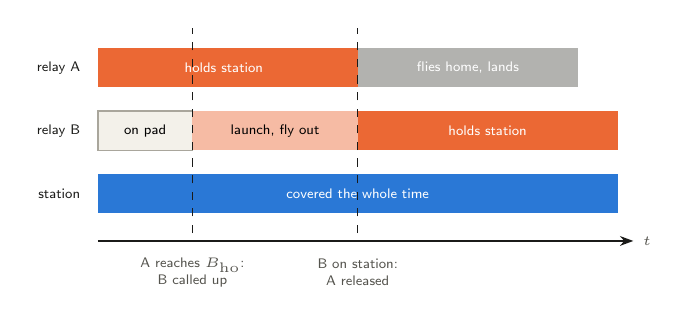
\begin{tikzpicture}[x=1mm,y=1mm]
  \node[lab,anchor=east,text=ink] at (13,21) {relay A};
  \node[lab,anchor=east,text=ink] at (13,13) {relay B};
  \node[lab,anchor=east,text=ink] at (13,5) {station};
  \fill[corange] (14,18.5) rectangle (47,23.5); \node[font=\sffamily\tiny,white] at (30,21) {holds station};
  \fill[ink2!45] (47,18.5) rectangle (75,23.5); \node[font=\sffamily\tiny,white] at (61,21) {flies home, lands};
  \fill[faint] (14,10.5) rectangle (26,15.5); \draw[rule] (14,10.5) rectangle (26,15.5); \node[font=\sffamily\tiny] at (20,13) {on pad};
  \fill[corange!45] (26,10.5) rectangle (47,15.5); \node[font=\sffamily\tiny] at (36.5,13) {launch, fly out};
  \fill[corange] (47,10.5) rectangle (80,15.5); \node[font=\sffamily\tiny,white] at (63.5,13) {holds station};
  \fill[cblue] (14,2.5) rectangle (80,7.5); \node[font=\sffamily\tiny,white] at (47,5) {covered the whole time};
  \draw[dashed] (26,0) -- (26,26); \draw[dashed] (47,0) -- (47,26);
  \draw[->] (14,-1) -- (82,-1) node[right,lab]{$t$};
  \node[lab,align=center] at (26,-5) {A reaches $B_{\mathrm{ho}}$:\\B called up};
  \node[lab,align=center] at (47,-5) {B on station:\\A released};
\end{tikzpicture}
\caption{Make-before-break. The overlap between the dashed lines is the price of never opening a gap; Eq.~(\ref{eq:ho}) sizes it so that A can afford to wait and still get home.}
\label{fig:handover}
\end{figure}

\subsection{Failover and routing}
\paragraph{Failover.} An aircraft is ``heard'' when anyone, another aircraft or the GCS, measures a usable link to it. A relay nobody has heard for 200\,ms is treated as failed, and the scout with the best score
\begin{equation}
e_i=\frac{b_i}{100}\,\bar q_i\,\rho_i
\label{eq:elect}
\end{equation}
is promoted into its slot, where $b_i$ is battery, $\bar q_i$ mean measured link quality and $\rho_i$ a role weight. The router recomputes at once. Detection dominates the latency (Fig.~\ref{fig:failover}): in our logged runs the whole thing, from silence to traffic on the new route, took 200 to 300\,ms. Nothing that still works is demoted. Our first election re-ranked the whole swarm on every failure, and we watched it push a healthy relay out of its role.

\begin{figure}[t]
\centering
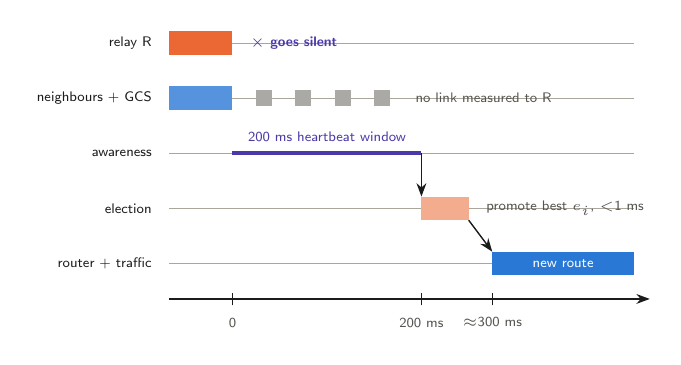
\begin{tikzpicture}[x=1mm,y=1mm]
  \foreach \y/\t in {30/relay R,23/neighbours + GCS,16/awareness,9/election,2/router + traffic}
    {\node[lab,anchor=east,text=ink] at (22,\y) {\t}; \draw[rule,line width=0.3pt] (23,\y) -- (82,\y);}
  \fill[corange] (23,28.5) rectangle (31,31.5); \node[font=\sffamily\tiny\bfseries,text=cviolet,anchor=west] at (32,30) {$\times$ goes silent};
  \fill[cblue!80] (23,21.5) rectangle (31,24.5);
  \foreach \x in {34,39,44,49} \fill[ink2!50] (\x,22) rectangle (\x+2,24);
  \node[lab,anchor=west] at (53,23) {no link measured to R};
  \draw[cviolet,line width=1.4pt] (31,16) -- (55,16); \node[lab,text=cviolet,anchor=south] at (43,16.3) {200 ms heartbeat window};
  \draw[->] (55,16) -- (55,10.5);
  \fill[corange!55] (55,7.5) rectangle (61,10.5); \node[lab,anchor=west] at (62,9) {promote best $e_i$, $<$1 ms};
  \draw[->] (61,7.5) -- (64,3.5);
  \fill[cblue] (64,0.5) rectangle (82,3.5); \node[font=\sffamily\tiny,white] at (73,2) {new route};
  \draw[->] (23,-2.5) -- (84,-2.5);
  \foreach \x/\t in {31/0,55/200 ms,64/$\approx$300 ms} {\draw (\x,-3.3) -- (\x,-1.7); \node[lab] at (\x,-5.5) {\t};}
\end{tikzpicture}
\caption{Failover as it happens. Nobody announces that R has failed. The swarm notices that nobody can hear it; after 200\,ms the election fills the slot and the router moves traffic. The election takes microseconds; the waiting is what costs time.}
\label{fig:failover}
\end{figure}

\paragraph{Routing.} Routes are shortest paths [14] over the flying ad-hoc network [4], with the GCS as a node, on a cost that mixes current quality with how stable the causal model expects a link to be:
\begin{equation}
c_{ij}=(1-\alpha)\big(-\log q_{ij}\big)+\alpha\big(-\log s_{ij}\big),\quad \alpha=0.3,
\label{eq:route}
\end{equation}
where $s_{ij}$ is an exponential average (weight 0.3) of $1-\hat L_{ij}$ from the SCM in Sec.~\ref{sec:scm}, halved while the link is anomalous. Taking logs makes the path cost the negative log of end-to-end reliability, so Dijkstra finds the most reliable route rather than the shortest.

\subsection{Traffic, acknowledgements and custody}
Packets actually move (Fig.~\ref{fig:traffic}). Every airborne aircraft sends telemetry at 2\,Hz, dropped once older than 2\,s, and each surveyed site produces 12 chunks of imagery and situational data. Each hop is link-layer ARQ with up to four tries, so a hop that succeeds on attempt $a$ costs
\begin{equation}
t_{\mathrm{hop}}=\sum_{k=0}^{a-1}\big(4.1+2k\big)\,\mathrm{ms}+1.5\,\mathrm{ms},
\label{eq:arq}
\end{equation}
where 4.1\,ms is the airtime of a 256-byte frame at about 500\,kbit/s. A bad link therefore shows up as latency before it shows up as loss. Survey chunks are delay-tolerant [7]: with no route they wait in custody on the aircraft holding them, and an aircraft that lands hands its backlog to the GCS over the wire. Every delivered packet is acknowledged, and those acknowledgements are the only way an aircraft knows it still has a link home. Sixty seconds without one triggers the lost-link return.

\begin{figure}[t]
\centering
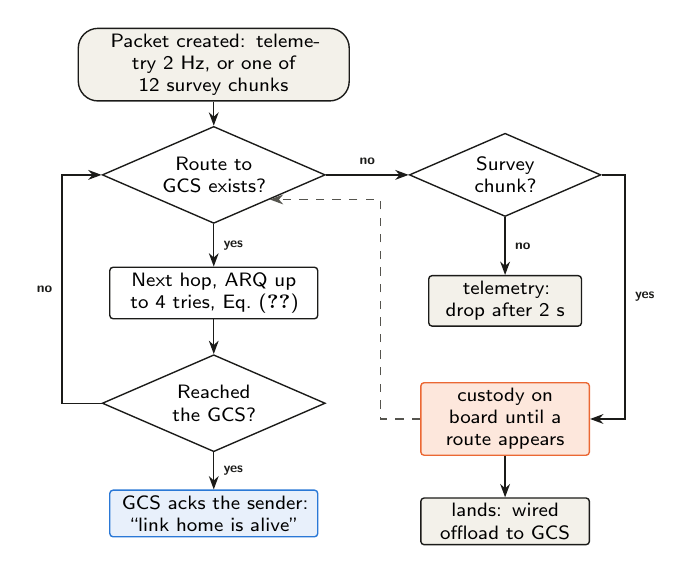
\begin{tikzpicture}[x=1mm,y=1mm]
  \node[term,text width=33mm] (g) at (0,0) {Packet created: telemetry 2 Hz, or one of 12 survey chunks};
  \node[dec,text width=17mm] (r) at (0,-14) {Route to GCS exists?};
  \node[bx,text width=25mm] (h) at (0,-29) {Next hop, ARQ up to 4 tries, Eq.~(\ref{eq:arq})};
  \node[dec,text width=17mm] (ok) at (0,-43) {Reached the GCS?};
  \node[bxb,text width=25mm] (ack) at (0,-57) {GCS acks the sender: ``link home is alive''};
  \node[dec,text width=13mm] (ty) at (37,-14) {Survey chunk?};
  \node[bxg,text width=18mm] (drop) at (37,-30) {telemetry: drop after 2 s};
  \node[bxo,text width=20mm] (cus) at (37,-45) {custody on board until a route appears};
  \node[bxg,text width=20mm] (land) at (37,-58) {lands: wired offload to GCS};
  \draw[arr] (g) -- (r);
  \draw[arr] (r) -- node[right,yes]{yes} (h);
  \draw[arr] (h) -- (ok);
  \draw[arr] (ok) -- node[right,yes]{yes} (ack);
  \draw[arr] (ok.west) -- ++(-5,0) |- node[pos=0.25,left,yes]{no} (r.west);
  \draw[arr] (r) -- node[above,yes]{no} (ty);
  \draw[arr] (ty) -- node[right,yes]{no} (drop);
  \draw[arr] (ty.east) -- ++(3,0) |- node[pos=0.25,right,yes]{yes} (cus.east);
  \draw[arr] (cus) -- (land);
  \draw[arr,ink2,dashed] (cus.west) -- ++(-5,0) |- (r.south east);
\end{tikzpicture}
\caption{The life of one packet. Acknowledgements double as the swarm's only evidence that it is still connected, which is what the lost-link failsafe listens to.}
\label{fig:traffic}
\end{figure}

\subsection{Safety}
Every setpoint is projected at least 40\,m inside the geofence and under the AGL ceiling before the controller sees it. Separation assurance predicts each pair's closest point of approach over the next 4\,s. With $\mathbf r$ and $\mathbf v$ the relative position and velocity (vertical axis weighted by 1.6),
\begin{equation}
t^\ast=\mathrm{clip}\Big(-\frac{\mathbf r\cdot\mathbf v}{\|\mathbf v\|^2},0,4\Big),\qquad d=\|\mathbf r+\mathbf v t^\ast\|.
\label{eq:cpa}
\end{equation}
If $d$ is under $R=30$\,m (8\,m near the pads), the pair is pushed apart along the miss vector by $0.9R(R-d)/R$ and split vertically, higher one up. The fence and terrain floor are then re-applied, so avoidance can never push an aircraft out of bounds. Take-offs are spaced 4\,s apart. In all 24 benchmark runs there were no collisions, geofence violations, terrain strikes or flat batteries.

% ================================================================= 6
\section{Knowing Without Being Told}\label{sec:scm}
A simulator makes cheating easy. The first version of this code, like many swarm demos, read the injected fault directly: ``if this drone is marked dead, re-elect''. That makes a fault look handled while a real swarm would still be finding out about it. We removed every such path. A disturbance now changes physics or radio and nothing else; no flag is set and no callback fires. Table~\ref{tab:dist} lists what the swarm actually sees. A test file audits the autonomy's source for any read of simulator state, and behavioural tests check that each disturbance is noticed rather than announced.

\begin{table}[t]
\centering
\caption{How each hidden disturbance is noticed.}
\label{tab:dist}
\footnotesize
\renewcommand{\arraystretch}{1.1}
\begin{tabularx}{\columnwidth}{@{}>{\raggedright\arraybackslash}p{15mm}>{\raggedright\arraybackslash}X>{\raggedright\arraybackslash}X@{}}
\toprule
\textsf{\textbf{Event}} & \textsf{\textbf{Evidence}} & \textsf{\textbf{Conclusion}}\\
\midrule
UAV failure & nobody hears it for 200 ms & failover; task freed after 5 s\\
Radio outage & same silence; own packets unacked & treated as failure; home after 60 s\\
Interference & noise-floor rise; DF bearings & source cross-fixed, fed to planning\\
Area RF drop, link cut & floor up everywhere; links fall & chain re-sized, re-routed\\
Motor or cell fault & current above thrust model & $\hat k$ rises: earlier RTH\\
Heavy rain & RSSI below map; camera loses ground & path-loss offset; cloud ceiling\\
GNSS drift & radio ranging disagrees & terrain-relative nav\\
New emergency & report reaches GCS & tasking, pre-emption\\
\bottomrule
\end{tabularx}
\end{table}

\paragraph{Estimators.} Beliefs are simple and cheap. Wind is an exponential average of the aircraft's own estimates (time constant 20\,s), scaled to cruise height by the shear law. The path-loss offset is $\delta\leftarrow\delta+0.3\,(\mathrm{med}(P^{\mathrm{map}}_r-P^{\mathrm{meas}}_r)-1-\delta)$ once a second over up to ten links, which is how rain is noticed. GNSS drift is caught when radio ranging to other aircraft and to the GCS disagrees with GNSS ranges by more than a threshold. Ranging to the GCS was added after we found that a drift common to every aircraft is invisible to ranging between aircraft.

\paragraph{Where is the interference?} Each receiver reports its noise floor, and a rise over 6\,dB counts as interference. Each aircraft's direction-finding array also reports bearings to strong emitters, with noise that grows as the signal weakens and a fixed calibration bias. The swarm scores candidate cells $\mathbf c$ on a grid by how well one emitter explains the readings. For aircraft $k$ in the active set $\mathcal A$ with measured interference $J_k$ and predicted path loss $\ell_k(\mathbf c)$ (free space plus terrain, from the map it carries),
\begin{equation}
\begin{gathered}
\hat P(\mathbf c)=\frac{1}{|\mathcal A|}\sum_{k\in\mathcal A}\big(J_k+\ell_k(\mathbf c)\big),\\
E(\mathbf c)=\sum_{k\in\mathcal A}\big(J_k+\ell_k(\mathbf c)-\hat P(\mathbf c)\big)^2+E_{\mathrm{silent}}+E_{\mathrm{DF}},
\end{gathered}
\label{eq:loc}
\end{equation}
where $E_{\mathrm{silent}}$ penalises cells that would have raised the floor at aircraft which heard \emph{nothing}, and $E_{\mathrm{DF}}$ scores how well the cell agrees with the measured bearings. A ridge that shields one aircraft is evidence here, not noise. The best cell, its power and an uncertainty radius go to the relay optimiser, which then plans around it (Fig.~\ref{fig:jam}).

\begin{figure}[t]
\centering
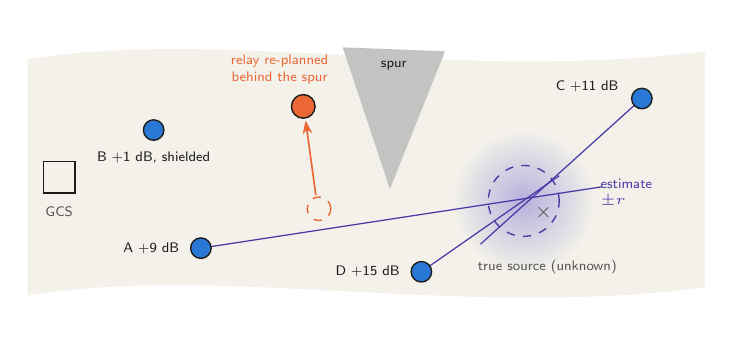
\begin{tikzpicture}[x=1mm,y=1mm]
  \fill[faint] (0,0) .. controls (25,4) and (55,-3) .. (86,1) -- (86,31) .. controls (55,27) and (25,34) .. (0,30) -- cycle;
  \fill[ink2!35] (40,31.5) -- (46,13.5) -- (53,31) -- cycle;
  \node[lab,text=ink,anchor=north] at (46.5,31) {spur};
  \filldraw[fill=faint,draw=ink] (2,13) rectangle (6,17); \node[lab,anchor=north] at (4,12.5) {GCS};
  \shade[inner color=cviolet!40,outer color=faint] (63,12) circle (9);
  \draw[cviolet,dashed] (63,12) circle (4.5);
  \node[text=ink2,font=\sffamily\scriptsize] at (65.5,10.5) {$\times$};
  \node[lab,anchor=north] at (66,5.8) {true source (unknown)};
  \draw[cviolet,line width=0.45pt] (22,6) -- (73,13.8);
  \draw[cviolet,line width=0.45pt] (50,3) -- (67.5,15.2);
  \draw[cviolet,line width=0.45pt] (78,25) -- (57.5,6.5);
  \foreach \x/\y/\n in {22/6/A,50/3/D,78/25/C,16/21/B} \filldraw[fill=cblue,draw=ink] (\x,\y) circle (1.3);
  \node[lab,text=ink,anchor=east] at (20.5,6) {A +9 dB};
  \node[lab,text=ink,anchor=east] at (48.5,3) {D +15 dB};
    \node[lab,text=ink,anchor=east] at (76.3,26.6) {C +11 dB};
  \node[lab,text=ink,anchor=north] at (16,19.5) {B +1 dB, shielded};
  \node[lab,text=cviolet,anchor=west,align=left] at (71.5,13) {estimate\\$\pm r$};
  \draw[corange,dashed] (37,11) circle (1.5);
  \filldraw[fill=corange,draw=ink] (35,24) circle (1.5);
  \draw[->,corange,line width=0.6pt] (36.6,12.7) -- (35.3,22.2);
  \node[lab,text=corange,anchor=south,align=center] at (32,25.6) {relay re-planned\\behind the spur};
\end{tikzpicture}
\caption{Localising interference from noise rises and DF bearings (purple). The swarm never sees the true source ($\times$). Its estimate, with a radius, enters the relay objective, which moves the relay so the spur sits between it and the source. B hears almost nothing, and that silence also counts as evidence.}
\label{fig:jam}
\end{figure}

\paragraph{Why is this link failing?} Low delivery on an important link could be terrain, range, interference, a bad antenna angle or weather, and the right response differs: climb, move closer, reroute, turn, or accept it. A structural causal model [6] relates normalised terrain occlusion $T$, distance $D$, noise rise $J$, antenna misalignment $\theta$ and weather $W$ to loss $L$ (Fig.~\ref{fig:scm}a):
\begin{equation}
L=\sigma\big(\beta_0+\beta_T T+\beta_D D+\beta_J J+\beta_\theta\theta+\beta_W W\big).
\label{eq:scm}
\end{equation}
The coefficients are tracked online by recursive least squares with forgetting factor $\lambda=0.98$ [13], using the sigmoid slope as a Gauss-Newton weight:
\begin{gather}
\mathbf K=\frac{\mathbf P\mathbf x}{\lambda+\mathbf x^\top\mathbf P\mathbf x},\quad
\boldsymbol\beta\leftarrow\Pi_{\mathcal B}\big[\boldsymbol\beta+\mathbf K\,(y-\hat y)\,\hat y(1-\hat y)\big],\label{eq:rls}\\
\mathbf P\leftarrow(\mathbf P-\mathbf K\mathbf x^\top\mathbf P)/\lambda .\nonumber
\end{gather}
$\Pi_{\mathcal B}$ clips each coefficient to its physical sign (more occlusion, range or noise can only hurt). Without it the regressors, which are strongly collinear in normal flight, let RLS slide to values that fit equally well and mean nothing. The root cause is the parent with the largest $|\beta_k X_k|$.

Correlation is not enough to justify a climb, so the swarm runs a small experiment. It records the loss, commands $\mathrm{do}(\Delta z)$ on the relay end of the link, and measures again (Fig.~\ref{fig:scm}b). The effect $\hat\tau=\bar L_{\mathrm{post}}-\bar L_{\mathrm{pre}}$ counts only if it exceeds 0.05 with $t\ge2$. If $J$ moved by more than 2.5\,dB or range by more than 8\% during the window, the test is confounded and reported as indeterminate rather than guessed. A null result escalates the climb from 15 to 30 to 60\,m before concluding ``not terrain'', since a 15\,m climb barely changes the geometry under a 600\,m ridge. Only one experiment runs at a time; overlapping climbs contaminated each other's measurements when we allowed more.

\begin{figure}[t]
\centering
\resizebox{\columnwidth}{!}{%
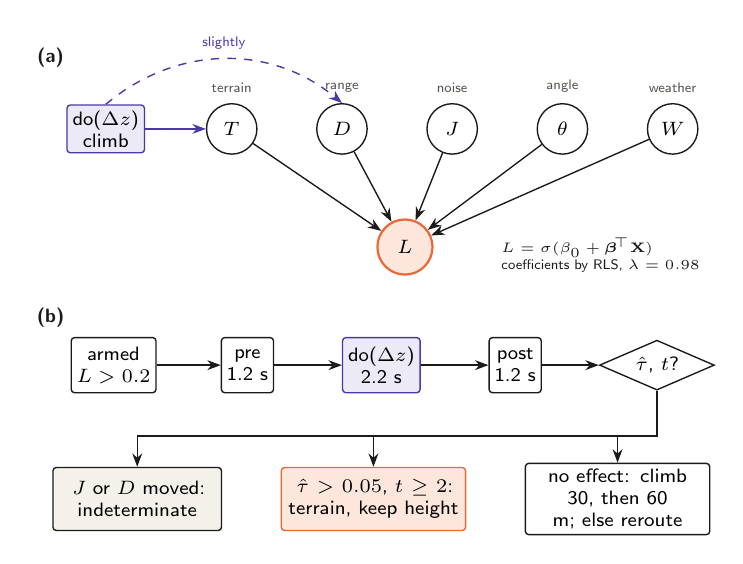
\begin{tikzpicture}[x=1mm,y=1mm]
  \node[lab,text=ink,font=\sffamily\scriptsize\bfseries] at (-15,31) {(a)};
  \foreach \n/\x/\t in {T/8/terrain,D/22/range,J/36/noise,Th/50/angle,W/64/weather}{
    \node[circle,draw=ink,fill=white,minimum size=6.4mm,inner sep=0] (\n) at (\x,22) {};
    \node[lab,anchor=south] at (\x,25.4) {\t};}
  \node at (T) {$T$}; \node at (D) {$D$}; \node at (J) {$J$}; \node at (Th) {$\theta$}; \node at (W) {$W$};
  \node[circle,draw=corange,fill=lorange,minimum size=7mm,inner sep=0,line width=0.8pt] (L) at (30,7) {$L$};
  \foreach \n in {T,D,J,Th,W} \draw[arr] (\n) -- (L);
  \node[bxv] (do) at (-8,22) {do($\Delta z$)\\climb};
  \draw[arr,cviolet,line width=0.7pt] (do) -- (T);
  \draw[arr,cviolet,dashed] (do.north) to[out=40,in=140] node[above,lab,text=cviolet,pos=0.5]{slightly} (D.north);
  \node[lab,anchor=west,align=left,text=ink] at (41,6) {$L=\sigma(\beta_0+\boldsymbol\beta^{\!\top}\mathbf X)$\\coefficients by RLS, $\lambda=0.98$};
  % lifecycle
  \node[lab,text=ink,font=\sffamily\scriptsize\bfseries] at (-15,-2) {(b)};
  \node[bx,minimum height=7mm] (a1) at (-7,-8) {armed\\$L>0.2$};
  \node[bx,minimum height=7mm] (a2) at (10,-8) {pre\\1.2 s};
  \node[bxv,minimum height=7mm] (a3) at (27,-8) {do($\Delta z$)\\2.2 s};
  \node[bx,minimum height=7mm] (a4) at (44,-8) {post\\1.2 s};
  \node[dec,text width=9mm] (a5) at (62,-8) {$\hat\tau$, $t$?};
  \draw[arr] (a1)--(a2); \draw[arr] (a2)--(a3); \draw[arr] (a3)--(a4); \draw[arr] (a4)--(a5);
  \node[bxg,text width=20mm,minimum height=8mm] (o1) at (-4,-25) {$J$ or $D$ moved:\\indeterminate};
  \node[bxo,text width=22mm,minimum height=8mm] (o2) at (26,-25) {$\hat\tau>0.05$, $t\ge2$:\\terrain, keep height};
  \node[bx,text width=22mm,minimum height=8mm] (o3) at (57,-25) {no effect: climb 30, then 60 m; else reroute};
  \draw (a5.south) -- (62,-17) -- (-4,-17);
  \draw[arr] (-4,-17) -- (o1.north); \draw[arr] (26,-17) -- (o2.north); \draw[arr] (57,-17) -- (o3.north);
\end{tikzpicture}}
\caption{(a) The structural causal model of link loss, with the altitude intervention acting on terrain occlusion. (b) One experiment. The swarm keeps a climb only when a clean, unconfounded measurement says terrain was the cause.}
\label{fig:scm}
\end{figure}

What we got from the experiments is honest but modest. The causal layer never blamed terrain for interference in our tests. It confirms genuine terrain shadow only about 20\% of the time, because climbing one end of a link lifts the ray over a far ridge by very little. The routing and interference layers do not depend on it being right; they use it as a stability hint.

Two more things surprised us. A relay whose radio fails and one that crashes look identical from outside, so the swarm handles both the same way; when the radio comes back the aircraft is heard, rejoins, and the role manager notices it has one relay too many. And honesty cost a little. When the energy model switched from the true wind to the swarm's own estimate, completion fell from 98.4\% to 93.5\%. The calibration had been fitted to ground-level wind, while the swarm now measures the stronger wind at cruise height. Refitting airspeed on the same logged flights brought it back to 97.3\%.

\begin{figure*}[t]
\centering
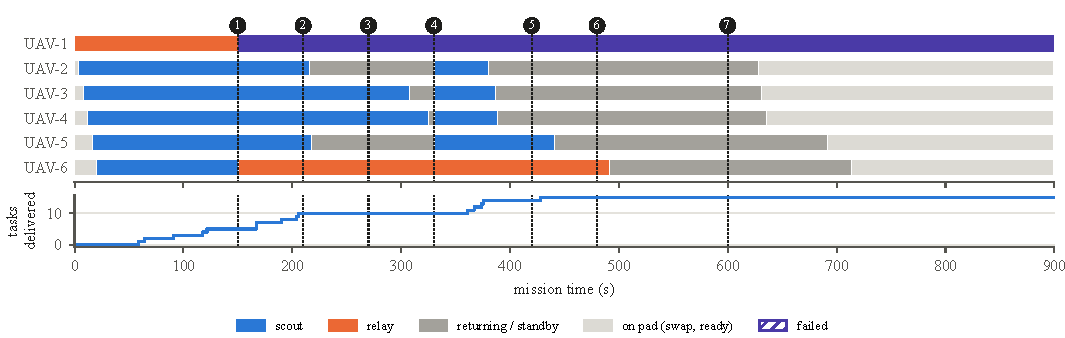
\includegraphics[width=\textwidth]{figs/fig_timeline.pdf}
\caption{One Kedarnath run, from its logs. Disturbances: \textbf{1} relay UAV-1 fails, \textbf{2} GCS receiver outage, \textbf{3} 30\% packet loss, \textbf{4} P1 region reported, \textbf{5} interference zone, \textbf{6} relay battery fault, \textbf{7} late P1 report. At 1 the swarm notices UAV-1's silence and promotes UAV-6 into its slot. At 4 two scouts heading home are turned round, and the region is delivered by about 430\,s. After 6 the faulty relay's measured drain rises and it comes home early. Event 7 arrives with 300\,s left and its round trip does not fit, so the planner declines it.}
\label{fig:timeline}
\end{figure*}

% ================================================================= 7
\section{Evaluation}\label{sec:eval}
\subsection{Scenarios, baseline and metrics}
A scenario is a JSON file fixing the terrain, seed, fleet, GCS, geofence, tasks, clock and a timeline of hidden disturbances. Positions can be given in metres or as a fraction along the valley, so one scenario runs on any site. The disturbance types cover everything listed for Stage~2. Table~\ref{tab:results} summarises the four we ship with their results.

The \textbf{baseline} keeps everything except the adaptive role layer: same flight control, energy-aware return, geofence, placement network and packet model. Roles are fixed at launch (one relay, the rest scouts) and aircraft relaunch in their original role. A failed relay is not replaced, a new P1 task waits for a free scout, nothing hands over and nobody stands by. The gap between the two is what the adaptive autonomy is worth. Each scenario runs with three seeds, which vary fading, packet outcomes and, in the stress case, task placement. Metrics follow the categories in the problem statement and are computed from simulator truth, never from what the swarm believes. The priority-weighted score is
\begin{equation}
S=\sum_p w_p\,\delta_p\Big/\sum_p w_p,
\label{eq:score}
\end{equation}
with $\delta_p=1$ if task $p$'s data reached the GCS by the deadline. Availability is airborne time with an end-to-end path of reliability at least 0.5; recovery time runs from a disruption until every airborne aircraft has had a path for 1\,s; reconfiguration efficiency is one minus the share of role changes undone within 30\,s.

\begin{table*}[t]
\centering
\caption{Scenarios and adaptive results per scenario (mean of three seeds). Tasks are those at launch plus those released later.}
\label{tab:results}
\footnotesize
\renewcommand{\arraystretch}{1.1}
\begin{tabular*}{\textwidth}{@{\extracolsep{\fill}}lrrrrrrrrr@{}}
\toprule
\textsf{\textbf{Scenario}} & \textsf{\textbf{UAVs}} & \textsf{\textbf{Tasks}} & \textsf{\textbf{Clock}} & \textsf{\textbf{Hidden events}} & \textsf{\textbf{Completion}} & \textsf{\textbf{PDR}} & \textsf{\textbf{Availability}} & \textsf{\textbf{Recovery}} & \textsf{\textbf{Min. battery}}\\
\midrule
Quickstart, synthetic valley & 5 & 8 + 1 & 12 min & 4 & 100.0\% & 95.4\% & 93.9\% & 4.6 s & 24.1\%\\
Kedarnath landslide (real terrain) & 6 & 10 + 6 & 15 min & 8 & 93.8\% & 97.2\% & 95.8\% & 8.9 s & 10.5\%\\
Uttarkashi earthquake (real terrain) & 5 & 9 + 6 & 15 min & 7 & 100.0\% & 100.0\% & 100.0\% & 0.0 s & 29.4\%\\
Stress, synthetic valley & 5 & 8 + 7 & 15 min & 11 & 95.6\% & 94.3\% & 91.5\% & 13.3 s & 21.3\%\\
\bottomrule
\end{tabular*}
\end{table*}

\begin{figure*}[t]
\centering
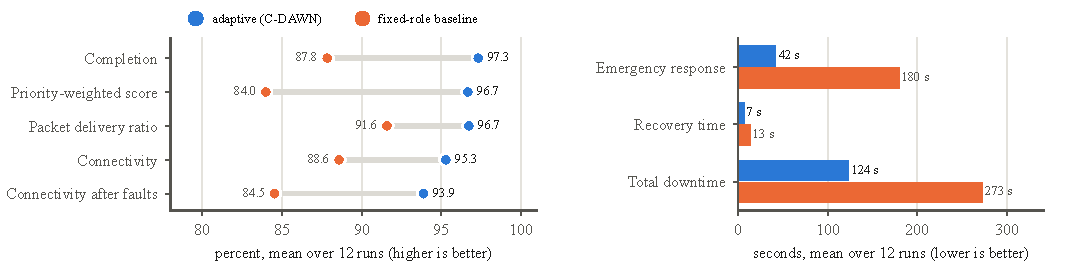
\includegraphics[width=\textwidth]{figs/fig_results.pdf}
\caption{Adaptive C-DAWN against the fixed-role baseline, mean of 12 runs each (4 scenarios $\times$ 3 seeds). Left: percentages (dots, since the axis is zoomed). Right: times in seconds. Neither strategy had a collision, a geofence violation or a flat battery.}
\label{fig:results}
\end{figure*}

\subsection{Results}
Fig.~\ref{fig:results} compares the two strategies over 12 runs each. The adaptive swarm is ahead on every mission and communication metric: completion 97.3\% against 87.8\%, priority-weighted score 96.7\% against 84.0\%, PDR 96.7\% against 91.6\% and availability 95.3\% against 88.6\%. The biggest gap is how quickly a new emergency is answered, 42\,s against 180\,s, because the baseline waits for a scout to become free while ours pre-empts one or turns one round. Downtime (124\,s against 273\,s) and recovery time (6.7\,s against 13.4\,s) are both roughly halved, because the chain is re-sized and re-staffed instead of being left as launched. After the first fault, availability stays at 93.9\% against 84.5\%.

Fig.~\ref{fig:timeline} follows one Kedarnath run, and Table~\ref{tab:results} breaks the numbers down. Uttarkashi is a draw with the baseline: the Bhagirathi valley there is straight and open, one relay covers everything, and adaptation has little to win, which is what it should look like. The stress scenario is hardest on communication; its 13\,s mean recovery is dominated by a 60\,s severed link and a 25\,s GCS outage that no re-planning can fix, only wait out. The adaptive swarm also flies its batteries harder, down to 10.5\% in Kedarnath against a baseline average of 34\%. That is still above the 8\% landing reserve, and it is the price of keeping aircraft working instead of parking them.


\subsection{What did not work}
Our first energy model was about 1.8 times too pessimistic and sent full-battery scouts home before they had done anything. Tasks were once left assigned to a scout that had died, so nobody else picked them up; they are now released after 5\,s of silence. A handover once never completed because the placement network kept moving the replacement away from the station it was meant to take, which is why a relay being relieved is now fixed in the plan. The liquid time-constant controller [5] we first proposed for flight control lost to a well-tuned cascaded PID in 16 of 16 paired gust trials (0.62\,m against 0.18\,m cross-track error), so the PID flies and the LTC runs in shadow.

% ================================================================= 8
\section{Software and Reproducibility}
The code is Python 3.10+ with PyTorch for the placement network, FastAPI and WebSockets for the GCS server, and React with Three.js for the operator console (Fig.~\ref{fig:dash}). Nothing needs a GPU or an internet connection once installed: terrain packs and trained weights ship in the repository. A live mission runs with \texttt{python run\_node.py --scenario kedarnath\_landslide --autostart}; a headless run at 5 to 9 times real time with \texttt{python run\_scenario.py scenarios/<name>.json}; and the full benchmark in Table~\ref{tab:results} with \texttt{python -m bench.uavx\_suite}.

\begin{figure}[t]
\centering
\fbox{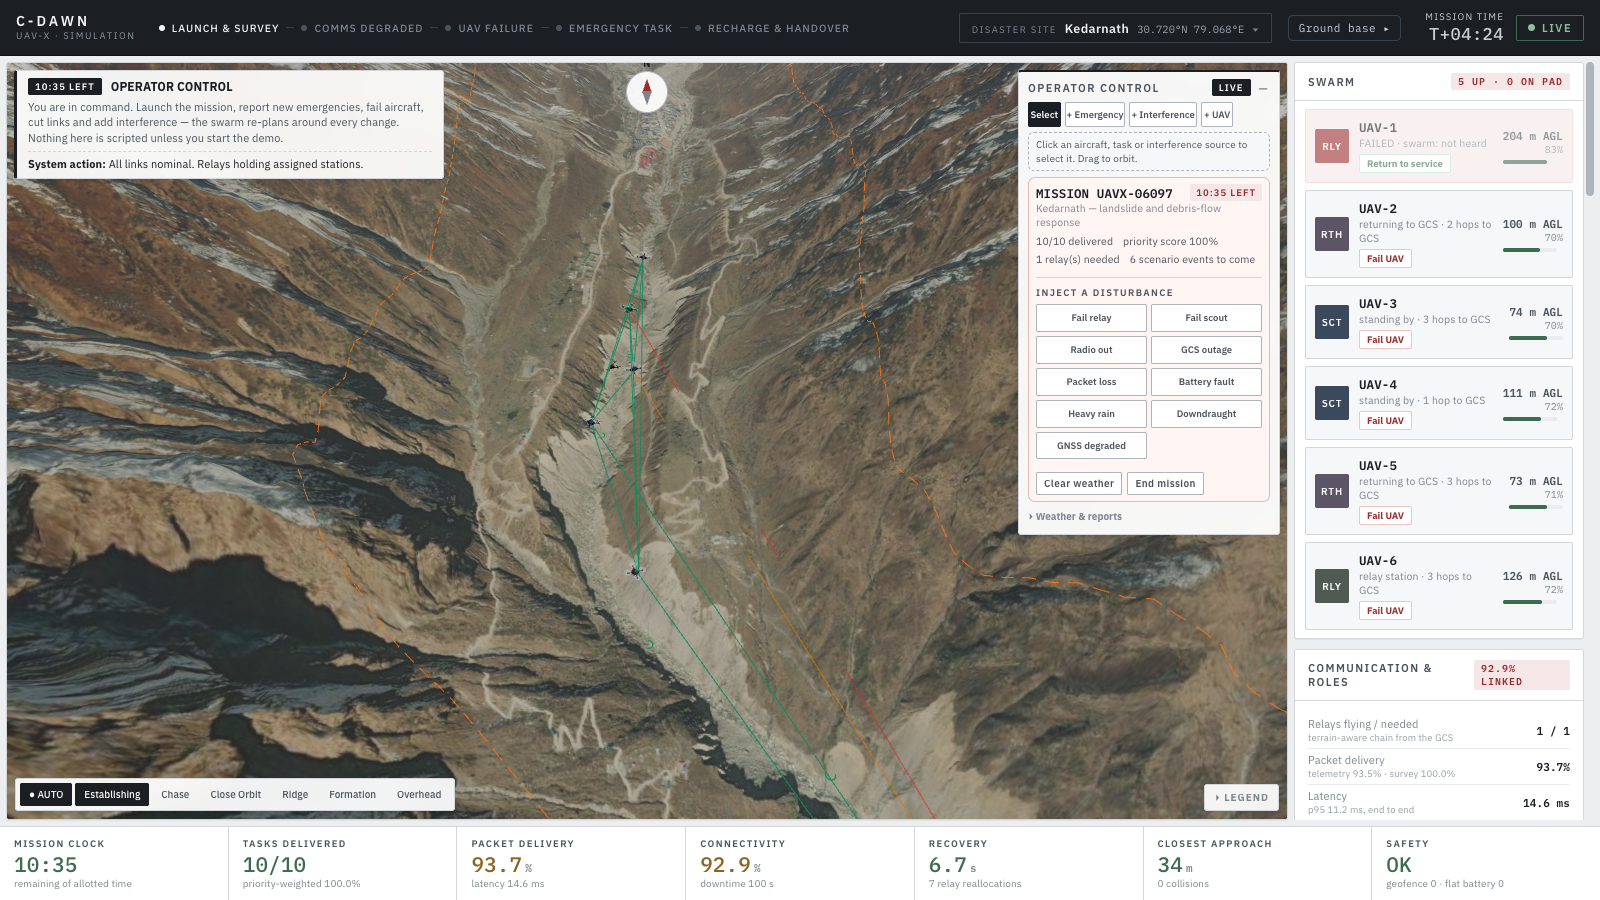
\includegraphics[width=\dimexpr\columnwidth-2\fboxsep-2\fboxrule]{figs/dashboard.png}}
\caption{The operator console during a live Kedarnath run: real terrain, geofence, relay chain, survey sites by priority, the swarm list with hop counts, and the challenge metrics along the bottom. Disturbances can be injected live from the same console.}
\label{fig:dash}
\end{figure}

The same code can be split across three laptops: one owns the aircraft and physics, one runs relay placement and causal diagnosis on the live stream, and one writes situation reports. Work falls back to the first if another goes quiet for 1.5\,s. Every run writes a standard log set (metadata with the code version, the resolved scenario, an event stream, 1\,Hz aircraft and link tables, a per-packet log and the metrics). When the organisers publish their log format, \texttt{mission/recorder.py} is the single adapter point. 158 automated tests cover physics, radio, GNN equivariance, failover, handover, traffic, every disturbance type and the truth-boundary audit.

% ================================================================= 9
\section{Limitations and Stage 2 Plan}
C-DAWN runs on its own simulator, which the problem statement allows in place of PX4, Gazebo or ns-3; it lets terrain, radio and flight share one model. The autonomy only ever talks to an aircraft through setpoints, so for Stage~2 we plan a PX4 SITL and ROS\,2 bridge that replaces the physics and controller hooks and leaves the autonomy untouched. Also on the list: a contention-aware MAC, since airtime is modelled per hop but not shared; the organisers' log format; position from a proper estimator rather than truth plus an injected GNSS offset; and air density that changes with altitude. Survey detections currently come from each site's category rather than imagery, and the situation reports are templates.

% ================================================================= 10
\section{Conclusion}
A swarm that surveys a disaster valley is only useful if what it sees gets home. By treating the link to the GCS as part of the mission, sizing the relay chain from the terrain, placing relays with a network trained through the physics itself, handing stations over before a battery forces the issue, and making the swarm find out about trouble the way a fielded one would, C-DAWN delivered 97\% of its tasks through 30 hidden disturbances without losing an aircraft to its own planning. The next step is the same autonomy on PX4, and after that on real airframes.

% ================================================================= refs
{\footnotesize
\setlength{\itemsep}{0pt}
\renewcommand{\refname}{References}
\begin{thebibliography}{14}\setlength{\itemsep}{0.5pt}
\bibitem{itu} ITU-R, ``Propagation by diffraction,'' Rec. P.526-15, 2019.
\bibitem{friis} H.\,T. Friis, ``A note on a simple transmission formula,'' \emph{Proc. IRE}, vol.\,34, no.\,5, pp.\,254 to 256, 1946.
\bibitem{egnn} V.\,G. Satorras, E. Hoogeboom and M. Welling, ``E(n) equivariant graph neural networks,'' in \emph{Proc. ICML}, 2021.
\bibitem{fanet} I. Bekmezci, O.\,K. Sahingoz and S. Temel, ``Flying ad-hoc networks (FANETs): A survey,'' \emph{Ad Hoc Networks}, vol.\,11, no.\,3, pp.\,1254 to 1270, 2013.
\bibitem{ltc} R. Hasani, M. Lechner, A. Amini, D. Rus and R. Grosu, ``Liquid time-constant networks,'' in \emph{Proc. AAAI}, 2021.
\bibitem{pearl} J. Pearl, \emph{Causality: Models, Reasoning and Inference}, 2nd ed. Cambridge Univ. Press, 2009.
\bibitem{dtn} K. Fall, ``A delay-tolerant network architecture for challenged internets,'' in \emph{Proc. ACM SIGCOMM}, 2003.
\bibitem{dryden} U.S. Department of Defense, ``Flying qualities of piloted aircraft,'' MIL-F-8785C, 1980.
\bibitem{dem} European Space Agency, ``Copernicus DEM,'' and AWS Open Data Terrain Tiles, accessed 2026.
\bibitem{s2} EOX IT Services, ``Sentinel-2 cloudless,'' s2maps.eu, CC BY 4.0.
\bibitem{sar} J. Scherer \emph{et al.}, ``An autonomous multi-UAV system for search and rescue,'' in \emph{Proc. ACM DroNet}, 2015.
\bibitem{adam} D.\,P. Kingma and J. Ba, ``Adam: A method for stochastic optimization,'' in \emph{Proc. ICLR}, 2015.
\bibitem{haykin} S. Haykin, \emph{Adaptive Filter Theory}, 5th ed. Pearson, 2014.
\bibitem{dijkstra} E.\,W. Dijkstra, ``A note on two problems in connexion with graphs,'' \emph{Numerische Mathematik}, vol.\,1, pp.\,269 to 271, 1959.
\end{thebibliography}}

\end{document}
